%-------------------------------------------------------
\section{Fundamentação Teórica}
%-------------------------------------------------------




%-------------------------------------------------------
    \begin{frame}{Análise de Revisão Sistemática}


        \Large
        % side by side text and figure
        \begin{columns}
            \begin{column}{0.65\textwidth}

                \begin{quadro}[htbp]
                    \centering
                    \caption{Referências mais citadas pelos documentos selecionados}
                    \label{quadro:citados}
                    \resizebox{.9\columnwidth}{!}{%
                    \begin{tabular}{p{0.45\linewidth}cp{\linewidth}}
                        \hline 
                        Referência citada & Citações & Visão Geral \\ \hline \hline
                        \citeauthor{markowitz1952portfolio} \citeyear{markowitz1952portfolio} & 31 & Teoria Moderna de Portfólio. \\ \hline
                        \citeauthor{almahdi2017adaptive}\citeyear{almahdi2017adaptive} & 8 & Alocação de carteira utilizando aprendizagem por reforço recorrente com máximo \textit{drawdown}. \\ \hline
                        \citeauthor{hochreiter1997long}\citeyear{hochreiter1997long} & 8 & Redes neurais recorrentes LSTM. \\ \hline
                        \citeauthor{kolm2014years}\citeyear{kolm2014years} & 8 & Revisão de 60 anos da teoria de otimização de portfólio. \\ \hline
                        \citeauthor{demiguel2009optimal}\citeyear{demiguel2009optimal} & 7 & Comparação de portfólio ótimo com modelo uniforme $1/N$. \\ \hline
                        \citeauthor{fischer2018deep}\citeyear{fischer2018deep} & 7 & Previsão de movimento de mercado com LSTM aplicado a grande dimensionalidade. \\ \hline
                        \citeauthor{sharpe1994sharpe}\citeyear{sharpe1994sharpe} & 7 & Índice de Sharpe. \\ \hline
                        \citeauthor{chen2021mean}\citeyear{chen2021mean} & 6 & Combina método de predição de aprendizagem de máquina XGBoost com modelo de média-variância para seleção de carteiras. \\ \hline
                        \citeauthor{heaton2017deep}\citeyear{heaton2017deep} & 6 & Revisão sobre o arcabouço de otimização de portfólio utilizando aprendizagem profunda. \\ \hline
                        \citeauthor{moody1998performance}\citeyear{moody1998performance} & 6 & Aprendizagem por reforço com aplicação do índice Sharpe com custos de transação para construção de carteiras. \\ \hline
                    \end{tabular}%
                    }
                    \par \footnotesize Fonte: próprio autor.
                \end{quadro}

            \end{column}
            \begin{column}{0.5\textwidth}

        
                \begin{figure}[htbp]
                    \centering
                    \caption{Mapa de co-citação dos artigos}
                    \label{fig:co_citacao}
                    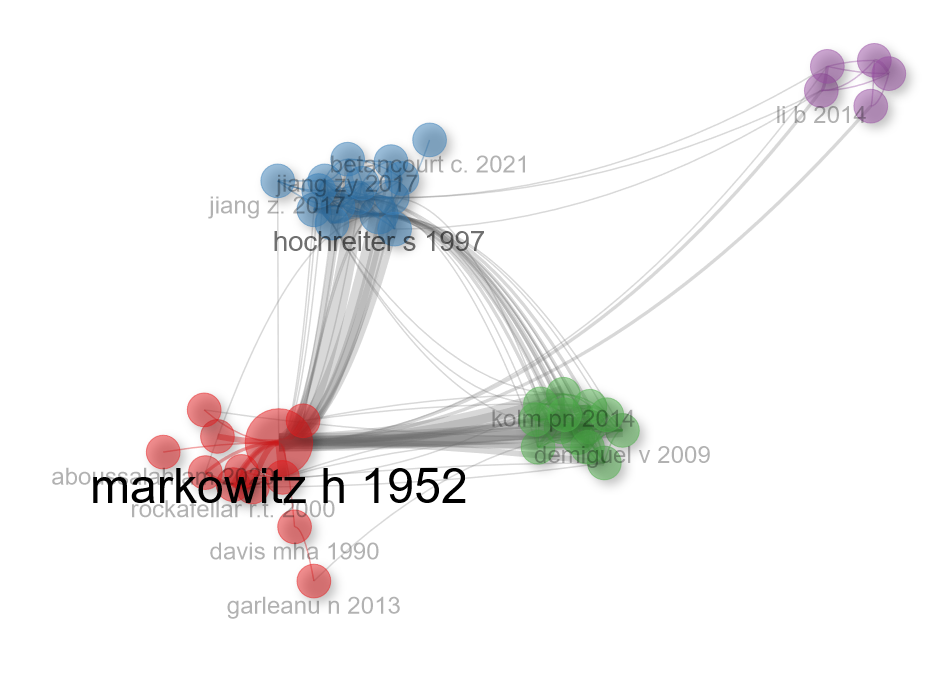
\includegraphics[width=0.98\textwidth]{./images/cocitation_network.png}
                    \par \footnotesize Fonte: próprio autor.
                \end{figure}

            \end{column}
        \end{columns}
        


    \end{frame}
    \note{Co-citação e referencias mais citadas}
%-------------------------------------------------------





%-------------------------------------------------------
    \begin{frame}{Risco e Retorno}

        \LARGE

        \begin{equation}
            \text{Retorno} = \frac{{P_f-P_i}}{{P_i}}
        \end{equation}

        % side by side text and figure
        \begin{columns}
            \begin{column}{0.3\textwidth}


                Retorno esperado:
                \begin{itemize}
                    \item Média
                    \item Média Móvel
                    \item Média Móvel Exponencial
                    \item Outros
                \end{itemize}

            \end{column}
            \begin{column}{0.3\textwidth}

                Risco:
                \begin{itemize}
                    \item Variância
                    \item Desvio Padrão
                    \item GARCH
                \end{itemize}

                \vspace{25pt}

            \end{column}

            \begin{column}{0.3\textwidth}

                Portfólio:
                \begin{itemize}
                    \item Média ponderada
                    \item Matriz de Covariância
                \end{itemize}

                \vspace{25pt}

            \end{column}
        \end{columns}
                

    \end{frame}
    \note{Média e variância}
%-------------------------------------------------------




%-------------------------------------------------------
    \begin{frame}{Otimização de Portfólio}


        \LARGE \textbf{Média e Variância}

        % side by side text and figure
        \begin{columns}
            \begin{column}{0.5\textwidth}

                \begin{equation}
                    \label{eq:markowitz}
                    \begin{aligned}
                        & \underset{w}{\text{minimizar}}
                        & & w^T \Sigma w \\
                        & \text{sujeito a}
                        & & w^T \mu = \mu_p \\
                        & & & w^T \mathbf{1} = 1 \\
                        & & & w \geq 0
                    \end{aligned}
                \end{equation}
        
            \end{column}
            \begin{column}{0.5\textwidth}

                \begin{figure}[htbp]
                    \centering
                    \caption{Otimização de portfólio utilizando o modelo de média-variância}
                    \label{fig:mínimo_risco}
                    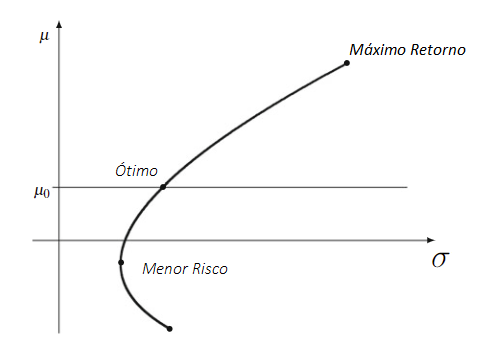
\includegraphics[width=0.6\textwidth]{images/minimo_risco.png}
                    \par \footnotesize Fonte: adaptado de \citeauthor{mansini2015linear}.
                \end{figure}
        
            \end{column}
        \end{columns}
        

    \end{frame}
    \note{Média e variância, Sharpe}
%-------------------------------------------------------





%-------------------------------------------------------
    \begin{frame}{Otimização de Portfólio}

        \LARGE \textbf{Aversão ao Risco}

        % side by side text and figure
        \begin{columns}
            \begin{column}{0.5\textwidth}

                \begin{equation}
                    \label{eq:aversao}
                    \begin{aligned}
                        & \underset{w}{\text{maximizar}}
                        & & w^T \mu - \lambda w^T \Sigma w \\
                        & \text{sujeito a} \\
                        & & & w^T \mathbf{1} = 1 \\
                        & & & w \geq 0
                    \end{aligned}
                \end{equation}
            \end{column}

            \begin{column}{0.5\textwidth}

                \begin{figure}[htbp]
                    \centering
                    \caption{Otimização de portfólio utilizando o modelo com o parâmetro $\lambda$ de aversão ao risco}
                    \label{fig:aversao}
                    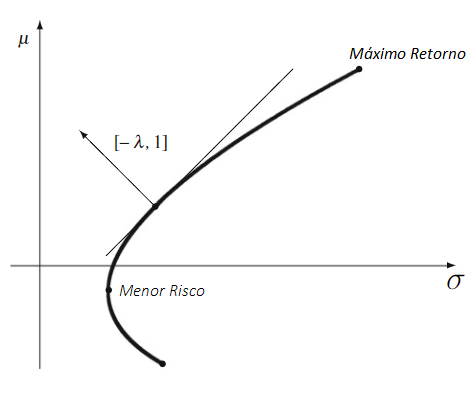
\includegraphics[width=0.6\textwidth]{images/aversao.png}
                    \par \footnotesize Fonte: adaptado de \citeauthor{mansini2015linear}.
                \end{figure}
        
            \end{column}
        \end{columns}

    \end{frame}
    \note{Outros modelos, restrições reais e heurística}
%-------------------------------------------------------




%-------------------------------------------------------
    \begin{frame}{Otimização de Portfólio}

        \LARGE \textbf{Maximização do Índice de Sharpe}

        % side by side text and figure
        \begin{columns}
            \begin{column}{0.5\textwidth}

                \begin{equation}
                    \label{eq:sharpe}
                    \begin{aligned}
                        & \underset{w}{\text{maximizar}}
                        & & \frac{w^T \mu - r_f}{\sqrt{w^T \Sigma w}} \\
                        & \text{sujeito a} \\
                        & & & w^T \mathbf{1} = 1 \\
                        & & & w \geq 0
                    \end{aligned}
                \end{equation}

            \end{column}

            \begin{column}{0.5\textwidth}

                    \begin{figure}[htbp]
                        \centering
                        \caption{Linha do mercado de capitais}
                        \label{fig:carteira_de_mercado}
                        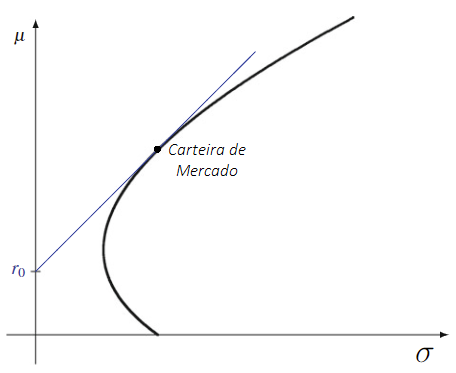
\includegraphics[width=0.6\textwidth]{images/carteira_de_mercado.png}
                        \par \footnotesize Fonte: adaptado de \citeauthor{mansini2015linear}.
                    \end{figure}
        
            \end{column}
        \end{columns}

    \end{frame}
    \note{Outros modelos, restrições reais e heurística}
%-------------------------------------------------------





%-------------------------------------------------------
    \begin{frame}{Otimização de Portfólio}

        \LARGE \textbf{Parâmetros Reais}

        \begin{itemize}
            \item Restrições de capital de investimento
            \item Custos de operação
            \item Cotação e lotes de negociação
            \item Rebalanceamento
            \item Cardinealidade
            \item Aversão ao risco
        \end{itemize}

        Problema de otimização não linear inteiro misto, NP-difícil.

    \end{frame}
    \note{Outros modelos, restrições reais e heurística}
%-------------------------------------------------------




%-------------------------------------------------------
    \begin{frame}{Redes Neurais}

        As Redes Neurais são modelos computacionais inspirados no funcionamento do cérebro humano, capazes de aprender e realizar tarefas complexas de processamento de informações.

        \begin{figure}[htbp]
            \centering
            \caption{Célula LSTM.}
            \label{fig:lstm}
            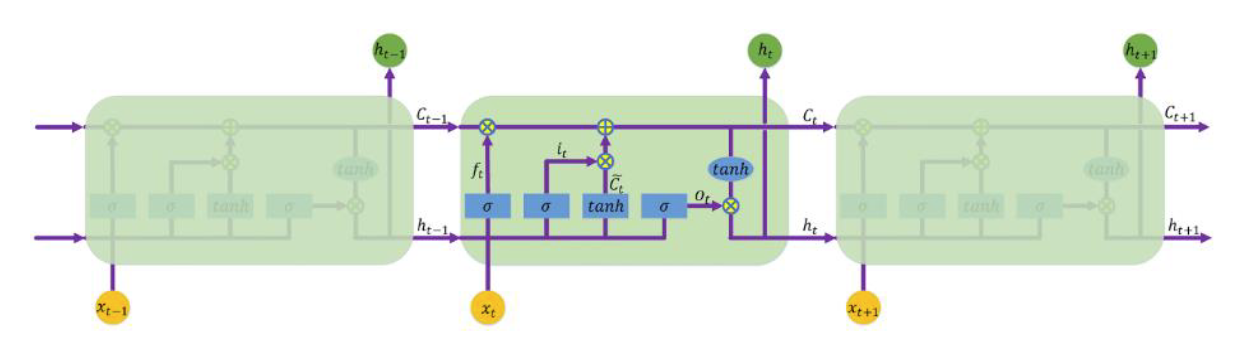
\includegraphics[width=0.95\textwidth]{images/lstm.png}
            \par \footnotesize Fonte: \citeauthor{ta2020portfolio}.
        \end{figure}


    \end{frame}
    \note{Principais métodos}
%-------------------------------------------------------





%-------------------------------------------------------
    \begin{frame}{Redes Neurais Recorrentes e Atenção}

        \Large
        % side by side text and figure
        \begin{columns}
            \begin{column}{0.5\textwidth}

                Mecanismo de atenção é capaz de capturar dependências de longo alcance entre origem e destino. Modelos:

                \begin{itemize}
                    \item Atenção Aditiva (\citeauthor{bahdanau2015neural})
                    \item Auto Atenção (\citeauthor{vaswani2017attention})
                \end{itemize}
                

            \end{column}

            \begin{column}{0.5\textwidth}

                \begin{figure}[htbp]
                    \centering
                    \caption{Mecanismo de atenção.}
                    \label{fig:attention}
                    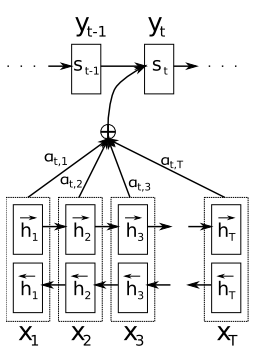
\includegraphics[width=0.5\textwidth]{images/attention.png}
                    \par \footnotesize Fonte: \citeauthor{bahdanau2015neural}.
                \end{figure}
        
        
            \end{column}
        \end{columns}


    \end{frame}
    \note{Arquitura e atenção}
%-------------------------------------------------------
